\section{Introducción}

Los algoritmos genéticos (AG) son una técnica de optimización inspirada en los principios de la evolución natural y la genética
basados en la mecánica de selección natural. Combinando la supervivencia del más apto con la reproducción sexual, con intercambio
de información estructurada \cite{marcos2010introduccion}. 

En la naturaleza, los organismos más aptos tienen una mayor probabilidad de sobrevivir y reproducirse, transmitiendo sus genes
a la siguiente generación. De manera similar, en los AG, las soluciones potenciales (individuos) se representan como cadenas de
caracteres (cromosomas) y se evalúan mediante una función de aptitud que mide su calidad. De tal manera que la combinación de buenos
ancestros puede generar descendencia aún mejor.

Estos algoritmos se utilizan para resolver problemas complejos mediante
la simulación de procesos evolutivos, como la selección, el cruce y la mutación. Los AG son especialmente útiles en problemas donde el espacio de búsqueda es grande y no se dispone de
una solución analítica directa.

\subsection{Conceptos Básicos}
\begin{itemize}
    \item \textbf{Población:} Conjunto de soluciones candidatas que evolucionan a lo largo del tiempo.
    \item \textbf{Generación:} Cada iteración del algoritmo, donde se aplican los operadores genéticos.
    \item \textbf{Cromosoma:} Representación de una solución en la población, comúnmente como una cadena de bits.
    \item \textbf{Alelo:} Valor específico que puede tomar un gen en un cromosoma.
    \item \textbf{Gen:} Elemento básico de un cromosoma, que representa una característica de la solución.
\end{itemize}

\begin{figure} [H]
    \centering
    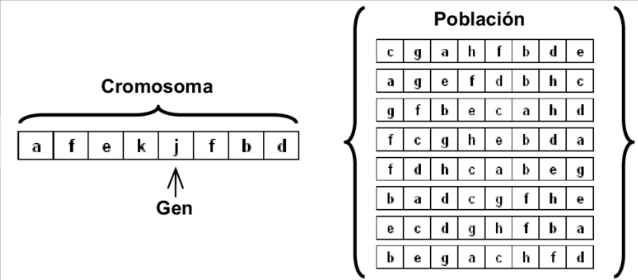
\includegraphics[width=0.5\textwidth]{C:/Users/death/Documents/Maestria/MCIA/Semestre_2/Metaheuristica/Reportes/Alg_Gen/rsc/img/genec.png}
    \caption{Representación de Poblacion y Cromosoma}
    \label{Poblacion}
\end{figure}

\subsection{Componentes de los Algoritmos Genéticos}
\begin{itemize}
    \item \textbf{Codificación de individuos:} Representación de las posibles soluciones del problema,
        comúnmente en forma de cadenas binarias, vectores o estructuras más complejas.
    
    \item \textbf{Función de aptitud (fitness):} Mide la calidad de cada individuo dentro de la población,
        es decir, qué tan buena es una solución respecto al objetivo del problema.
    
    \item \textbf{Población inicial:} Conjunto de individuos generados aleatoriamente o a partir de
        heurísticas, que servirán como punto de partida para la evolución.
    
    \item \textbf{Operadores genéticos:}
    \begin{itemize}
        \item \textbf{Selección:} Proceso mediante el cual se eligen los individuos que participarán en la reproducción, 
            favoreciendo a los de mayor aptitud.
            \begin{itemize}
                \item \textbf{Selección por torneo:} Se seleccionan aleatoriamente varios individuos y se elige el mejor entre ellos.
                \item \textbf{Selección por ruleta:} Cada individuo tiene una probabilidad de ser seleccionado proporcional a su aptitud.
                \item \textbf{Selección por rango:} Los individuos se ordenan según su aptitud y se asignan probabilidades de selección basadas en su posición en el ranking.
            \end{itemize}
        \item \textbf{Cruzamiento (crossover):} Combina el material genético de dos padres para generar descendencia con
            características de ambos.
            \begin{itemize}
                \item \textbf{Cruzamiento de un punto:} Se selecciona un punto de corte en los cromosomas de los padres y se intercambian las partes posteriores a ese punto.
                \item \textbf{Cruzamiento de k puntos:} Se seleccionan k puntos de corte y se intercambian las secciones entre esos puntos.
                \item \textbf{Cruzamiento aritmético:} Se combinan los valores de los padres mediante una operación aritmética (por ejemplo, promedio).
                \item \textbf{Cruzamiento de orden:} Utilizado en problemas de permutación, donde se preserva el orden relativo de los genes.
                \item \textbf{Cruzamiento de ciclo:} También para problemas de permutación, donde se identifican ciclos en los cromosomas de los padres para crear hijos.
                \item \textbf{Cruzamiento basado en la posición:} Se seleccionan posiciones específicas en los cromosomas de los padres para formar el hijo.
                \item \textbf{Cruzamiento de mezcla:} Se combinan segmentos de los padres de manera aleatoria.
            \end{itemize}
        \item \textbf{Mutación:} Introduce variaciones aleatorias en los individuos para mantener la diversidad genética y
            evitar la convergencia prematura.
    \end{itemize}
    
    \item \textbf{Criterios de paro:} Condiciones que determinan el final de la ejecución del algoritmo, como alcanzar un 
        número máximo de generaciones o una solución suficientemente buena.
\end{itemize}

\begin{figure}[H]
    \centering
    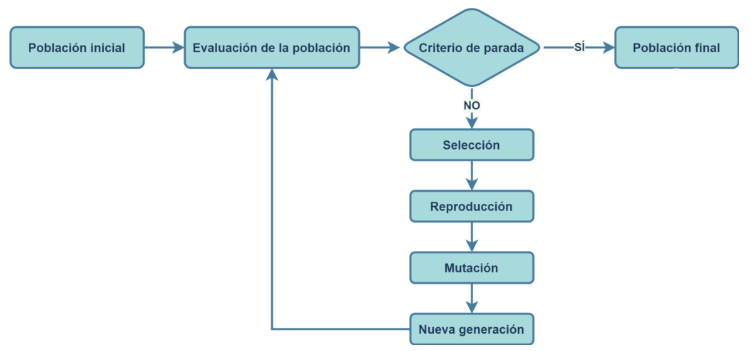
\includegraphics[width=0.8\textwidth]{C:/Users/death/Documents/Maestria/MCIA/Semestre_2/Metaheuristica/Reportes/Alg_Gen/rsc/img/Diagrama.png}
    \caption{Ciclo de un Algoritmo Genético}
    \label{diag}
\end{figure}

\subsection{Aplicacion a Algoritmo Dicotómico}

Para nuestro problema, desarrollaremos un AG que busque los mejores individuos según nuestra función de aptitud, la cual es $f(x) = x^2$.
Por lo tanto tomaremos en cuenta los siguientes aspectos:

\begin{itemize}
    \item Aptitud entre 0 y 1.
    \item Cromosoma: Binario de 6 bits.
    \item Alelos: 0 y 1.
    \item Función de aptitud: $f(x) = x^2$.
    \item Espacio de búsqueda: \{-1, 1\}[0, 63].
\end{itemize}

\begin{figure} [H]
    \centering
    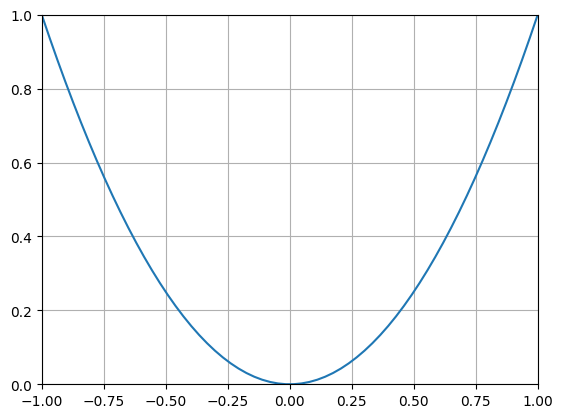
\includegraphics[width=0.5\textwidth]{C:/Users/death/Documents/Maestria/MCIA/Semestre_2/Metaheuristica/Reportes/Alg_Gen/rsc/img/funcion.png}
    \caption{Funcion de Aptitud $f(x) = x^2$}
    \label{funcion}
\end{figure}